\section{Simulations}
\label{sec:sim}

Our simulations assume two prey species and five time points, throughout.  Of the hierarchy of hypotheses, we generate data under three models: $c, c_s, c_t$.  Sample sizes for both prey species and predator gut count observations are randomly chosen from four overlapping levels: ``small'' sample sizes are randomly sampled numbers in $[20,50]$, ``medium'' $[30,75]$, ``large'' $[50,150]$, and ``huge'' $[100,200]$.  This is repeated for each level of sample size.  We simulate $500$ replicate datasets for each of the twelve scenarios above for both types of data, fully observed count data, $X_{jst}$, and for non-count data, when we observe only a binary response, $Z_{jst} = 1(X_{jst}>0)$.  Each scenario is then fit with the true model that generated the data.  All simulations of non-count data use $\tau = 10^{-5}$ as the convergence tolerance.  A subset of the examples are provided here; the interested reader is referred to the supplementary materials for the complete simulation results.  For the simulations we used the \texttt{R} \cite{Core-Team:2014} package \texttt{BatchExperiments} by \cite{Bischl:2014}.

For all simulated data, the true parameter values for the rate at which prey species are encountered in the wild are fixed to be $\gamma_{st} = \pi, \, \forall s,t$. The values of $\lambda_{st}$ are set with respect to each data generating model.  For model $c_{st} = c$, where predator preferences don't vary by either time or species, we put $\lambda_{st} = 2\pi, \forall s,t$.  Under model $c_s$, the ratio of rates vary by species only, so we put $\lambda_{1t} = \sqrt{2}$ and $\lambda_{2t} = \pi$.  Hence, $c_1 = \sqrt{2}/\pi \approx 0.45$ and $c_2 = 1$.  For the last model, $c_t$, the ratio of rates vary by time $t$.  Here, we put $\lambda_{st} = t$ for $t \in \{1, \ldots, 5 \}$.  

\begin{figure}
  \centering
  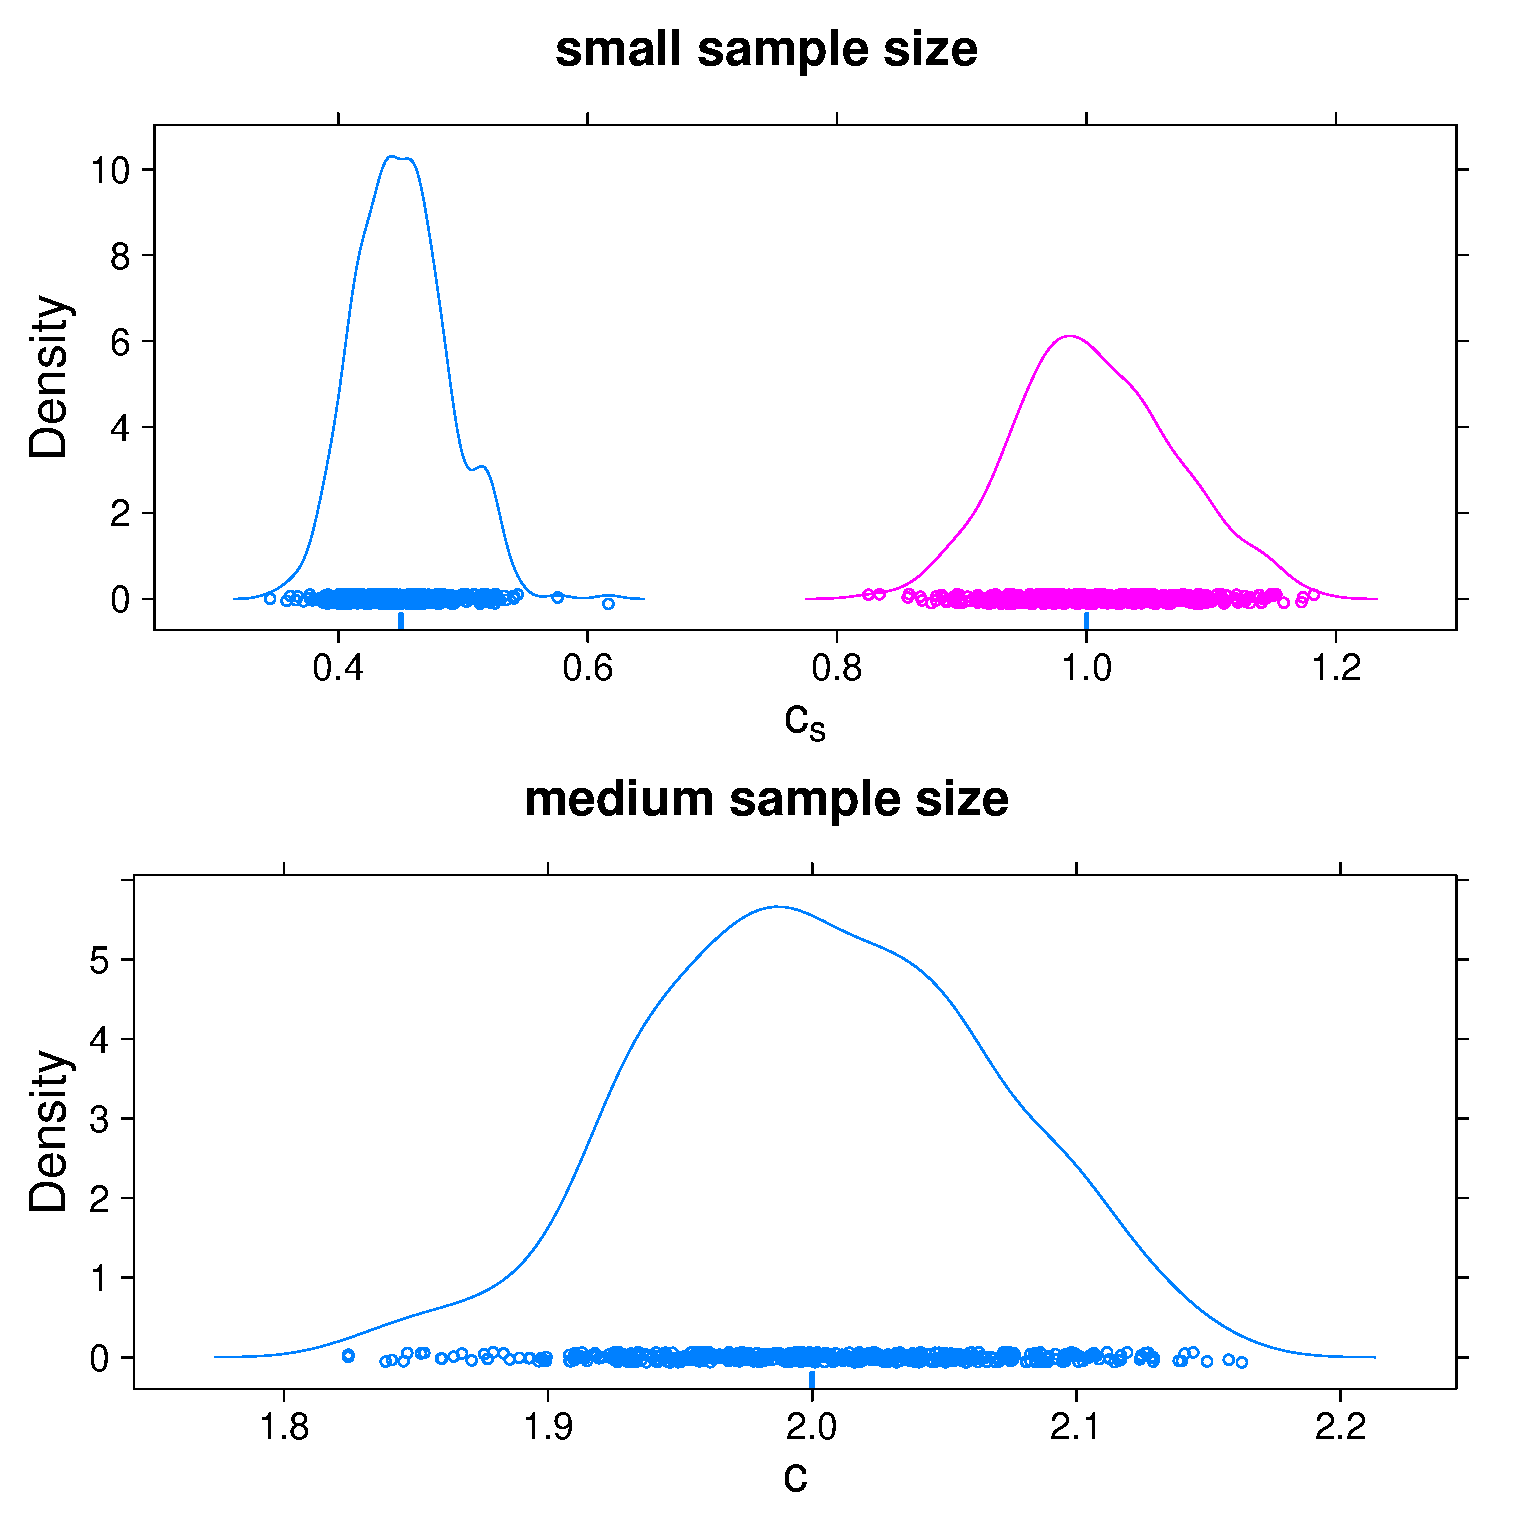
\includegraphics[scale=0.5]{nonem}
  \caption{Density plots of all $500$ estimates of fitting the true model to the data generated from models $c_s,c$ are shown with sample sizes small and medium, respectively.}
  \label{fig:nonem}
\end{figure}

Figure~\ref{fig:nonem} shows density plots of the estimates of $c_s, c$ when fitting the true model to the fully observed count data generated under models $c_s$ and $c$.  The plots provide evaluations of parameter estimates under each scenario.  In the first display, the parameters $c_1 \approx 0.45$ and $c_2 = 1$ are on average, across all $500$ simulations, estimated as $\hat{c}_1 = 0.45$ and $\hat{c}_2 = 1.00$, with standard errors of $\text{se}(\hat{c}_1) = 0.03$ and $\text{se}(\hat{c}_2) = 0.06$.  The second display provides results for model $c_{st} = c$.  Averaging across all $500$ simulations, the parameter $c=2$ is estimated as $\hat{c} = 2.00$.  This is further seen in figure~\ref{fig:bp}, where box plots of the parameter estimates, centered at true parameter values, of the correct model fit to data generated from both $c_s$ and $c_t$ show empirically very little bias.

\begin{figure}
  \centering
  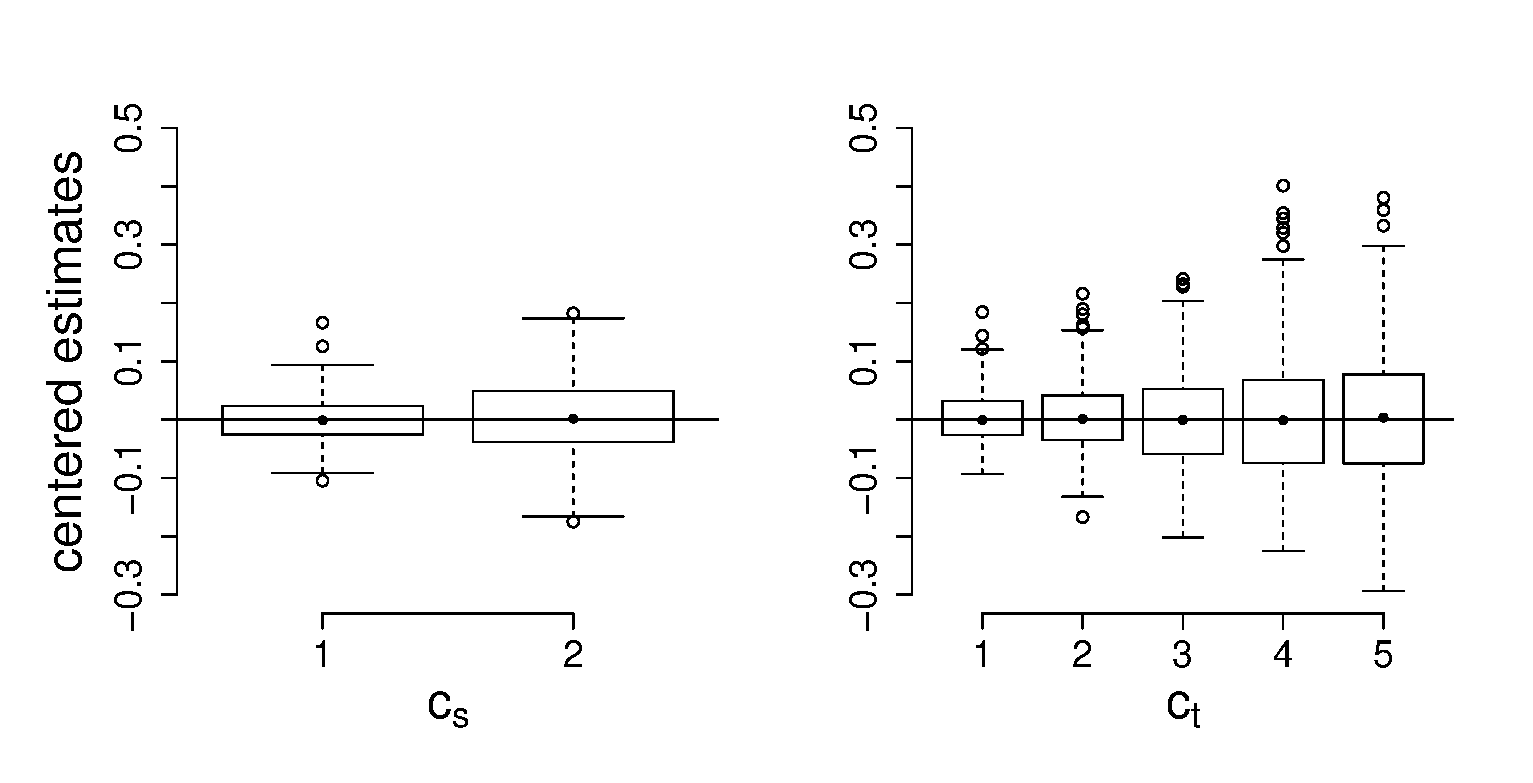
\includegraphics[scale=0.5]{bp}
  \caption{Shown are all $500$ estimates, centered at the true parameter values, from fitting the true model to the data generated from models $c_s,c_t$ with sample sizes small and medium, respectively.}
  \label{fig:bp}
\end{figure}

We next generated data with unobserved counts.  As noted above under certain circumstances our unobserved counts model accurately estimates the parameters of interest, and at other times can infinitely over-estimate parameters.  To investigate this issue further, we consider the same scenarios mentioned above, but now we reduce all of the count data down to binary observations.  For each scenario, we fit the unobserved counts model as if we knew the true underlying model that generated the observed data.

Figure~\ref{fig:em} contains density plots for all $500$ replications of the data generating models $c_s,c_t$ with small and huge sample sizes, respectively.  When data are generated under the model $c_s$ and the true model fit to the non-count data, we find even for the small sample size that point estimates are only very slightly biased.  When parameter values are of sufficient size to make zeros in the simulated data less common, the estimates from fitting the correct model to the generated data are occasionally over-estimated.  This effect is easily seen in the bottom panel of figure~\ref{fig:em} for larger values of $c_t$ despite the increased sample size, but is also seen, less dramatically, in the density plot for the $c_s$ generated data.  

The cluster of estimates for $c_5$ between $3.5$ and $4.0$ in the bottom panel of figure~\ref{fig:em} comes from datasets in which $X_{js5}>0$ so that $Z_{js5}=1$ for all $j,s$.  For the data shown in figure~\ref{fig:em}, this happened $73$ times out of the $500$ replicated datasets.  As mentioned above, the estimate of $c_5$ is infinite in this case. However, the EM algorithm will always provide a finite estimate for all parameters when it terminates.  In this case, we set $\tau=10^{-5}$ and it just happened that this caused the algorithm to terminate with $\hat c_5$ between $3.5$ and $4.0$.  To confirm that this is due to the arbitrary choice of $\tau$, we repeated the algorithm with smaller values of $\tau$ for several datasets. As expected, $\hat c_5$ increased without bound as we refit the model with increasingly small values of $\tau$.

\begin{figure}
  \centering
  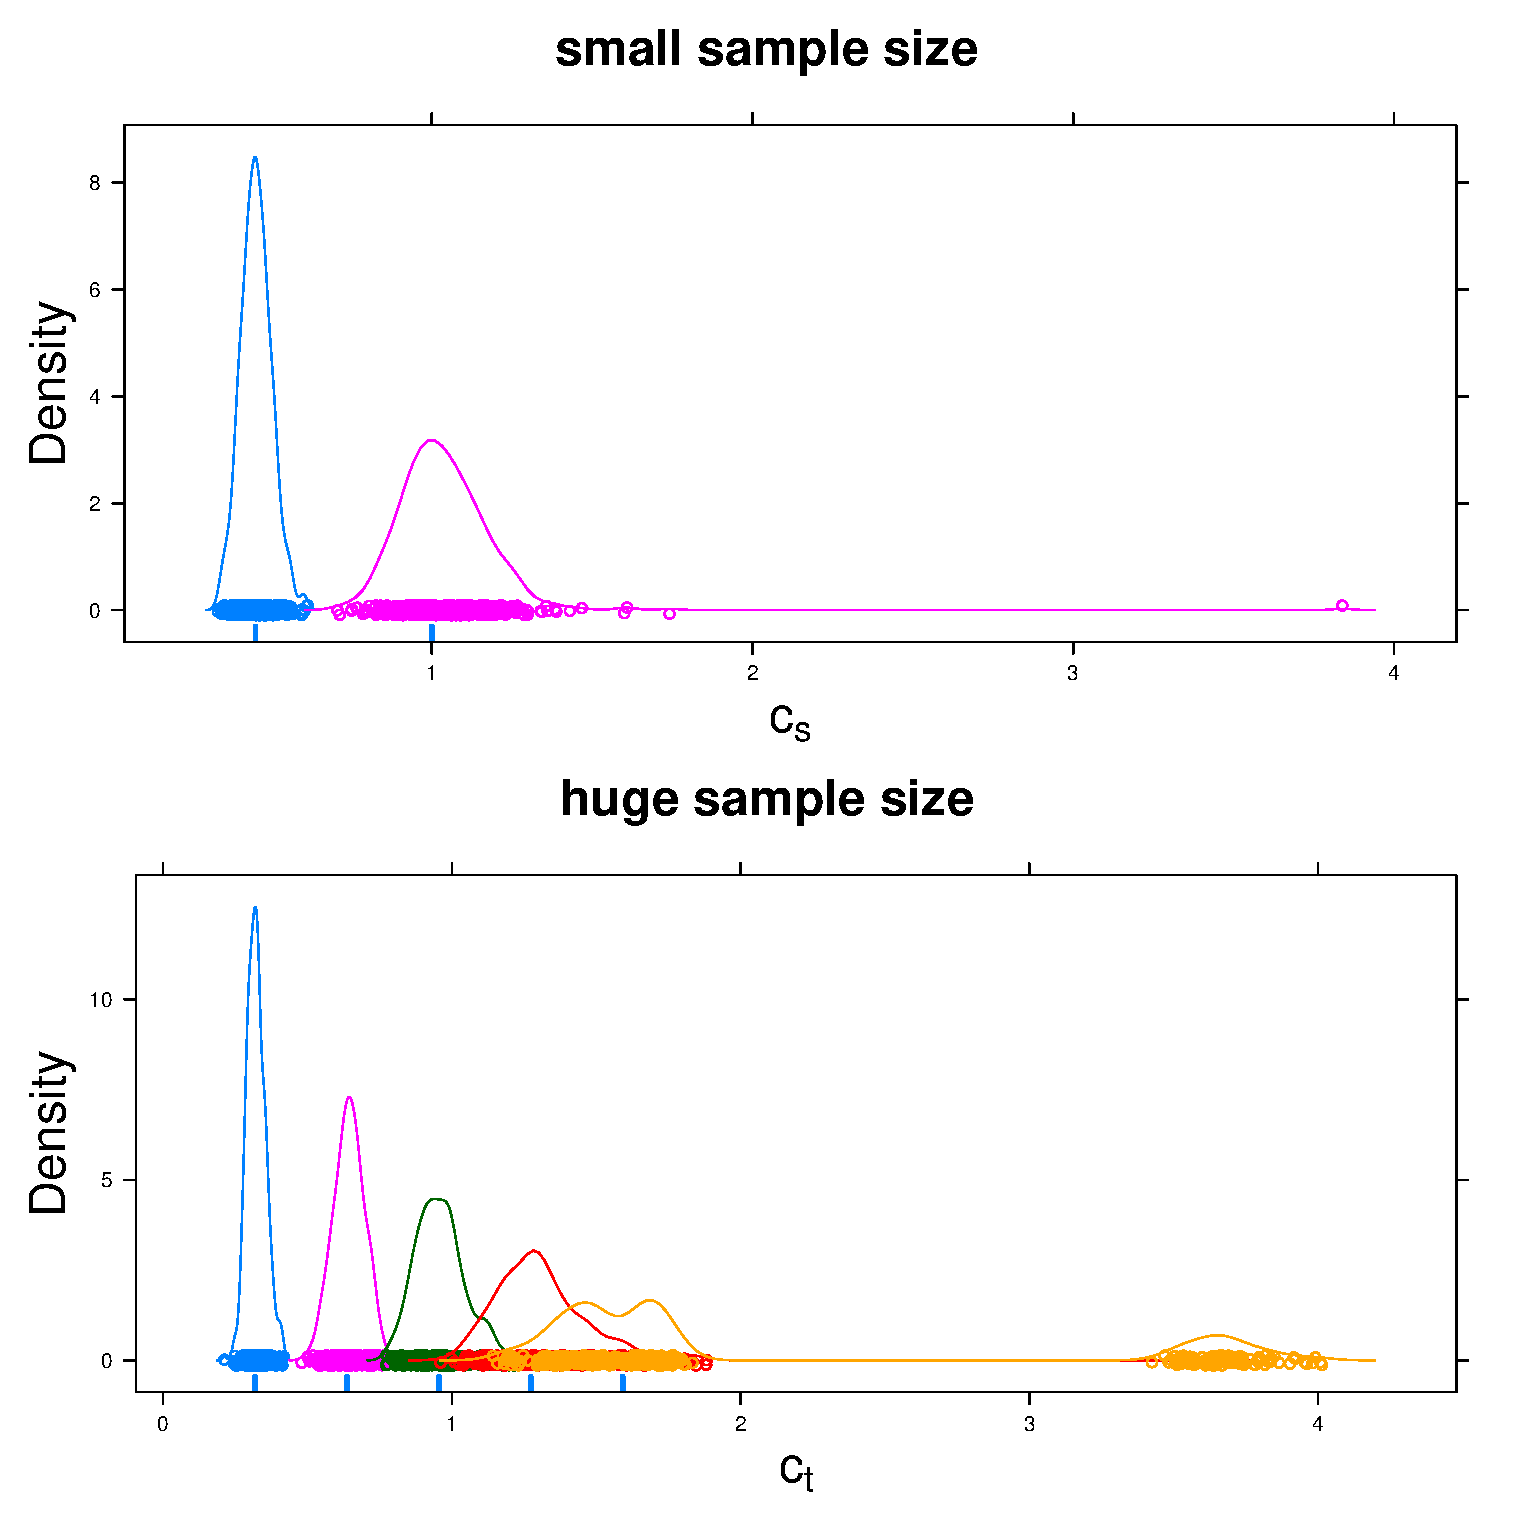
\includegraphics[scale=0.5]{em}
  \caption{Density plots of all $500$ estimates of fitting the true model to the data generated from models $c_s,c_t$, when counts are not observed, are shown with sample sizes small and huge, respectively.}
  \label{fig:em}
\end{figure}

The over-estimation of parameters, a symptom of the loss of information due to the unobserved counts, can also be seen with box plots of the $500$ point estimates centered at their respective true parameter values.  Figure~\ref{fig:em_bp} contains box plots of the same scenarios in Figure~\ref{fig:em}.  For the $73$ cases in which $Z_{js5} = 1$ for all $j,s$ under model $c_t$ with the huge sample size, the bias is infinite since parameter estimates will, theoretically, be infinite.  The finite bias shown in these plots is due to the finite estimates provided by the termination of the EM algorithm.  Thus, conditional on a mixture of $0$s and $1$s in the data the corresponding estimators are unbiased, but when no $0$s exist in the data the theoretical bias is infinite.  

\begin{figure}
  \centering
  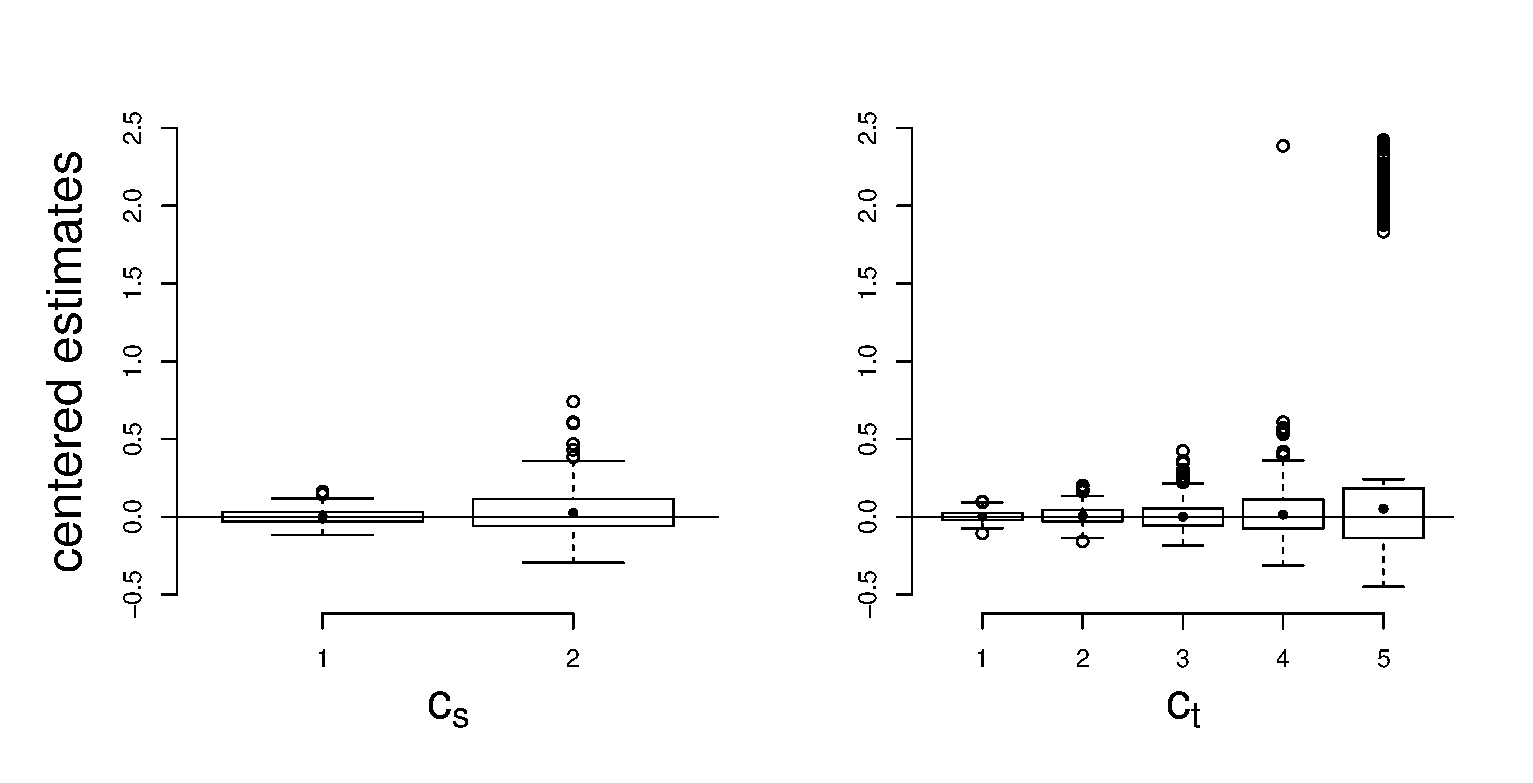
\includegraphics[scale=0.5]{em_bp}
  \caption{Shown are all $500$ estimates, centered at the true parameter values, from fitting the true model to the data generated from models $c_s,c_t$, when counts are not observed, with sample sizes small and huge, respectively.}
  \label{fig:em_bp}
\end{figure}

%%% Local Variables: 
%%% mode: latex
%%% TeX-master: "main"
%%% End: 
